\documentclass[compress]{beamer}
\usepackage[utf8]{inputenc}
\usepackage{hyperref}

\usepackage{tikz}
\usetikzlibrary{graphs, quotes, arrows.meta, matrix}

\usetheme{default}
\usecolortheme{Nord}
\setbeamertemplate{navigation symbols}{}

\title{More on graphs}
\subtitle{Binary Lifting, Cycle Detection e Cammini Euleriani}
\author{Lorenzo Ferrari, Davide Bartoli}
\date{\today}

\begin{document}

\begin{frame}
    \maketitle
\end{frame}

\begin{frame}{Table of contents}
  \tableofcontents
\end{frame}

\section{Binary Lifting}
\subsection{Grafi funzionali}
\begin{frame}{Binary Lifting}{Problema motivazionale}
    \begin{block}{Definizione: Grafo funzionale}
        Si dice \textbf{grafo funzionale} un grafo in cui ogni nodo  esattamente un arco uscente.
        Gli archi sono nella forma $(v, nxt(v))$ per qualche funzione $nxt: V \to V$
    \end{block}
        \pause
    \begin{exampleblock}{Binary Lifting}
        Dato un grafo funzionale $G$ con $N \leq 2 \cdot 10^5$ nodi, rispondi a $Q \leq 2 \cdot 10^5$ query che ti chiedono dove si trova il nodo $x$ dopo $K \leq 10^9$ step.
        \vfill
        \small{\underline{\url{https://cses.fi/problemset/task/1750/}}}
    \end{exampleblock}
    \pause
    \begin{itemize}
        \item idee?
    \end{itemize}
\end{frame}

\subsection{Idea e implementazione}
\begin{frame}{Binary Lifting}{Idea}
    Un'opzione \`e visitare uno alla volta i successori di $x$
    \pause
    \begin{itemize}
        \item questa soluzione \`e ovviamente troppo lenta
        \item la complessit\`a \`e $O(Q K)$
    \end{itemize}
    \pause
    \vfill
    Possiamo ottimizzare? Supponiamo di costruire un altro grafo funzionale $G'$ con gli archi $(v, nxt(nxt(v)))$. Il $K/2$-esimo successore di $x$ in $G'$ \`e il $K$-esimo successore di $x$ in $G$\footnote{questo \`e \textit{quasi} vero, dobbiamo fare attenzione a $K$ dispari}. \\

    \pause
    \vfill
    Cos\`i impieghiamo $K/2$ salti per raggiungere il $K$-esimo successore.

    \pause
    \vfill
    Notiamo che il problema per $G'$ \`e analogo al problema originale, continuiamo a usare la stessa ottimizzazione!
\end{frame}

\begin{frame}{Binary Lifting}{Implementazione}
    Sia $up[v][j]$ il $2^j$-esimo successore di $v$. $up[v][j]$ indica un salto lungo $2^j$.
    \begin{itemize}
        \item $up[v][0] = nxt(v)$
        \item $up[v][i] = up[up[v][i-1]][i-1] \ \forall i \geq 1$
    \end{itemize}
    \vfill
    \pause
    Per rispondere a una query, consideriamo $K$ nella sua rappresentazione binaria e costruiamo $K$ come composizione di salti lunghi $2^j$ per $O(\log K)$ valori di $j$.
    \vfill
    \begin{itemize}
        \item complessit\`a di tempo: $O((Q + N) \log K)$
        \item complessit\`a di spazio: $O(N \log K)$
    \end{itemize}
\end{frame}

\begin{frame}{Implementazione}
    \makebox[\textwidth]{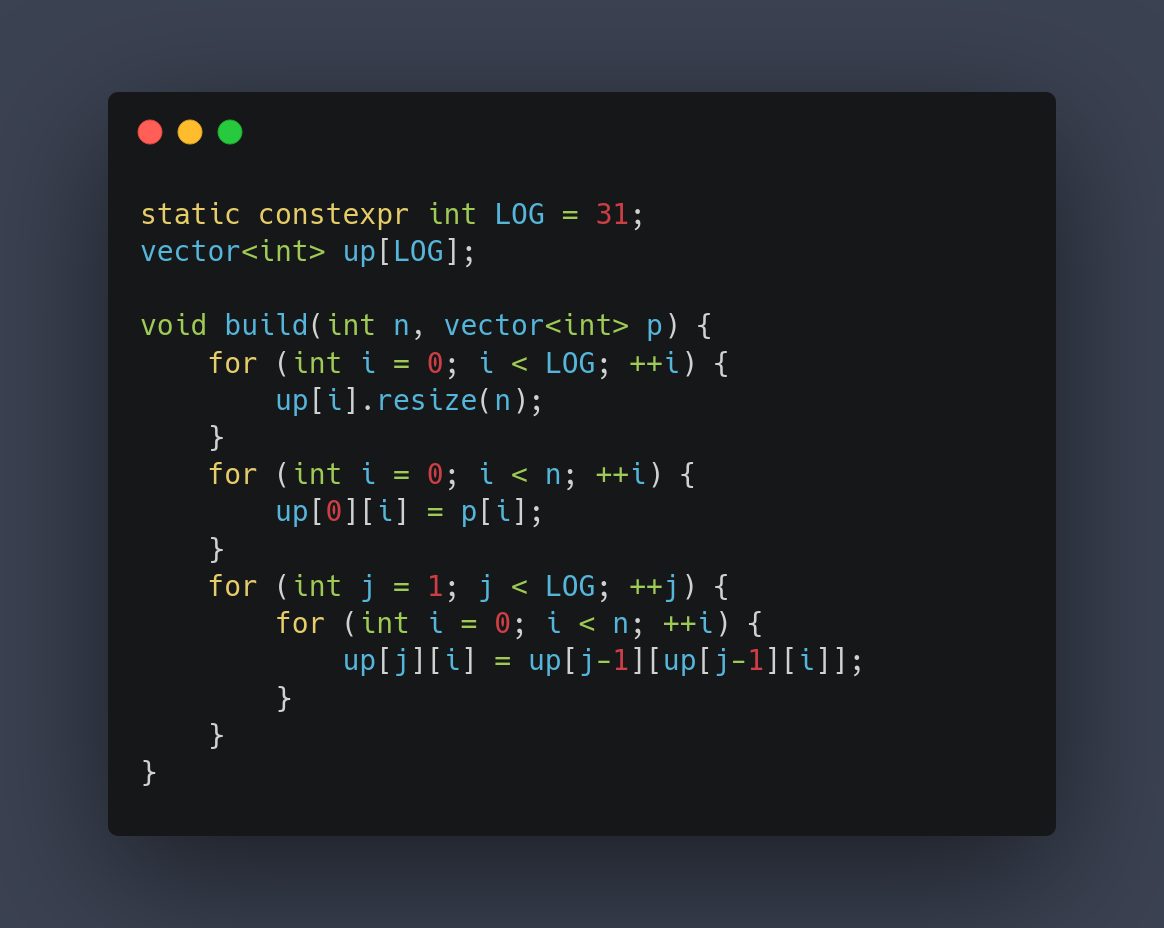
\includegraphics[scale=.25]{./img/lift_build.png}}
\end{frame}

\begin{frame}{Implementazione}
    \makebox[\textwidth]{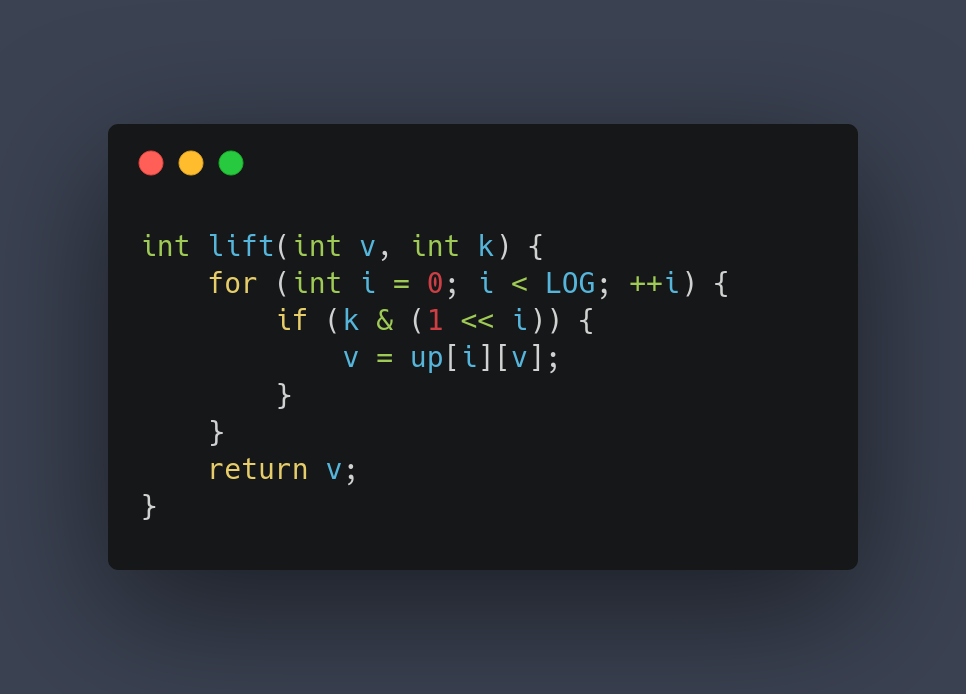
\includegraphics[scale=.3]{./img/lift_query.png}}
\end{frame}

\subsection{Lowest Common Ancestor}
\begin{frame}{Binary Lifting}{Lowest Common Ancestor}
    \begin{exampleblock}{LCA}
    Dato un albero radicato con $N \leq 2 \cdot 10^5$ nodi, trova per $Q$ coppie di nodi $(a, b)$ il loro minimo antenato comune.
        \vfill
        \small{\underline{\url{https://training.olinfo.it/\#/task/lca/statement}}}
    \end{exampleblock}
    \pause
    \begin{itemize}
        \item idee?
        \pause
        \item \textbf{algoritmo naive}
            \begin{itemize}
                \item alziamo il nodo pi\`u profondo fino all'altezza dell'altro
                \item finch\`e $a, b$ non coincidono, $a := nxt(a), b := nxt(b)$
                \item $a,b$ si incontrano nell'lca
            \end{itemize}
        \pause
    \item la complessit\`a al momento \`e $O(n)$ per query
    \end{itemize}
    \makebox[\textwidth]{
\includegraphics[scale=.08]{./img/not_stonks.jpg}}
\end{frame}

\begin{frame}{Binary Lifting}{Lowest Common Ancestor}
    Possiamo velocizzare entrambi gli step dell'algoritmo naive con \textbf{binary lifting}.
    \pause
    \begin{itemize}
        \item calcoliamo la profondit\`a $dep[v]$ di ogni nodo
        \item (wlog) il nodo $b$ \`e pi\`u profondo del nodo $a$
        \item $b := lift(b, dep[b] - dep[a])$
        \item se $a = b$, l'lca \`e $a$
        \item altrimenti raggiungiamo in $\log N$ salti i nodi $a',b'$ appena sotto l'lca
            \begin{itemize}
                \item (approfondiamo nell'implementazione)
            \end{itemize}
    \end{itemize}
    \pause
    Complessit\`a di tempo: $O(\log N)$ per query
\end{frame}

\begin{frame}{LCA}{Implementazione}
    \makebox[\textwidth]{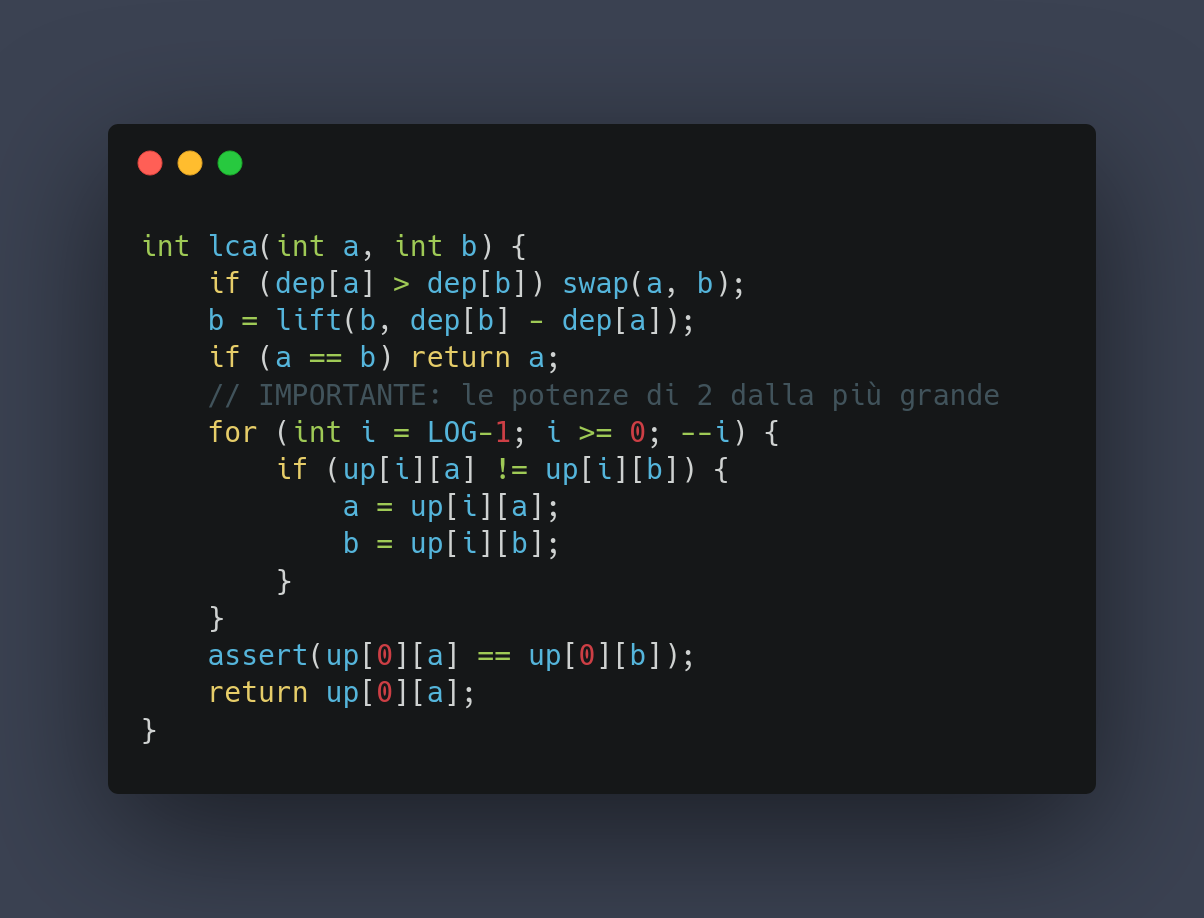
\includegraphics[scale=.25]{./img/lca.png}}
\end{frame}

\begin{frame}{LCA}{Varianti}
    Analogamente al segment, anche la \textbf{Sparse Table} per binary lifting \`e molto versatile.
    \pause
    \begin{alertblock}{}
        Purch\'e non ci siano update.
    \end{alertblock}
    \vfill
    \pause
    In generale, possiamo usare una generica struct \texttt{nodo} calcolabile da due nodi figli. Per esempio, possiamo rispondere a query di minimo/massimo/somma di un percorso, subarray con somma massima ecc.
    \vfill
    \small{\underline{\url{https://training.olinfo.it/\#/task/lca/statement}}}
\end{frame}

\section{Cycle Detection}
\subsection{Cicli in un grafo diretto}
\begin{frame}{Cycle Detection}{Problema}
    \begin{exampleblock}{Cycle Detection 1}
        Dato un grafo diretto con $N \leq 2 \cdot 10^5$ nodi e $M \leq 5 \cdot 10^5$ archi, stampare, se esiste, un ciclo.
    \end{exampleblock}
    \pause
    \begin{itemize}
        \item idee?
        \pause
        \item pensiamo a come funziona la DFS. In ogni momento i nodi possono essere:
        \begin{enumerate}
            \item attivi
            \item non attivi e non ancora visitati
            \item non attivi e gi\`a visitati
        \end{enumerate}
    \end{itemize}
    \begin{block}{Osservazione chiave}
        Se in un qualsiasi momento uno dei nostri vicini \`e un nodo attivo, allora siamo in un ciclo.
    \end{block}
\end{frame}

\subsection{Cicli negativi}
\begin{frame}{Cycle Detection}{Problema}
    \begin{exampleblock}{Cycle Detection 2}
        Dato un grafo pesato con $N \leq 2500$ nodi e $M \leq 5000$ archi, dire se esiste un ciclo con peso negativo.
        \small{\underline{\url{https://cses.fi/problemset/task/1197/}}}
    \end{exampleblock}
    \pause
    \begin{itemize}
        \item ricordiamo che l'algoritmo di Dijkstra non termina se il grafo contiene un ciclo negativo
        \item soluzione ``sbagliata'': facciamo Dijkstra, se \`e troppo lento esiste un ciclo negativo e lo fermiamo
        \pause
    \item soluzione legit: controlliamo se l'algoritmo di \textbf{Bellman-ford} va oltre la $(n-1)$-esima iterazione
    \end{itemize}
\end{frame}

\section{Cammini Euleriani}
\subsection{oii\_matita}
\begin{frame}{Cammini Euleriani}{Problema}
    \begin{exampleblock}{Cammino Euleriano}
        Dato un grafo non diretto, trova, se esite, un cammino euleriano, ovvero un cammino che passa per ogni arco esattamente una volta.
    \small{\underline{\url{https://training.olinfo.it/\#/task/oii_matita/statement}}}
    \end{exampleblock}
    \vfill
    \pause
    Come prima cosa cerchiamo di capire quando un cammino euleriano esiste.\\
    \pause
    \vfill
    Consideriamo un singolo nodo. Se il numero di archi incidenti \`e pari, allora il numero di volte che "entriamo" 
    nel nodo \`e uguale al numero di volte che "usciamo" dal nodo, quindi questo nodo può essere "nel mezzo" del nostro cammino.\\
    \pause
    Se invece il numero di archi incidenti \`e dispari, allora il nodo deve essere per forza il nodo da cui partiamo o il nodo in cui finiamo.\\
\end{frame}

\begin{frame}{Cammini Euleriani}
    Ora quindi sappiamo controllare se il cammino esiste: se il numero di nodi con grado dispari \`e $0$ o $2$, allora il cammino esiste, altrimenti no.\\
    \pause
    \vfill
    Come facciamo a trovare il cammino però?\\
    \pause
    \vfill
    In realtà \`e semplice, basta fare una dfs mantenedo l'array dei visitati sugli archi invece che sui nodi.\\
\end{frame}

\begin{frame}{Cammini Euleriani}{Implementazione}
    \makebox[\textwidth]{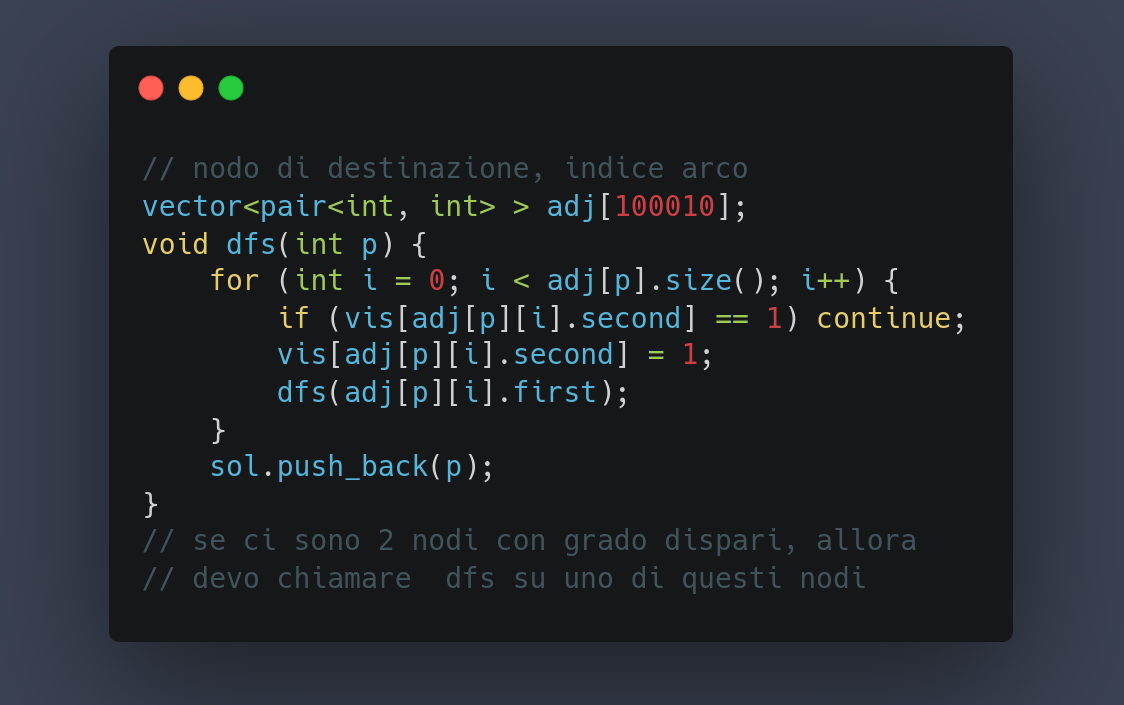
\includegraphics[scale=.25]{./img/eulerian.png}}
\end{frame}

\begin{frame}{Cammini Euleriani}
    Vedere perch\'e il codice funziona non è ovvio, bisogna ragionarci un pochino.\\
    \pause
    Possiamo fare alcune osservazioni:\\
    \begin{itemize}
        \item costruiamo il cammino in ordine inverso
        \pause
        \item se troviamo un cammino fino al nodo finale, quello che succede è che mentre "torniamo indietro" aggiungiamo 
        dei cicli che passano per il nodo corrente
        \pause
        \item utilizziamo sempre tutti gli archi (se rispetta le condizioni del cammino euleriano)
    \end{itemize}
    \pause
\end{frame}

\section{Problemi}
\begin{frame}{Problemi}
    \small{\underline{\url{https://cses.fi/problemset/task/1750/}}}
    \small{\underline{\url{https://cses.fi/problemset/task/1160/}}}
    \small{\underline{\url{https://cses.fi/problemset/task/1197/}}}
    \small{\underline{\url{https://training.olinfo.it/\#/task/oii_matita/statement}}}
    \small{\underline{\url{https://training.olinfo.it/\#/task/nostar/statement}}}
    \small{\underline{\url{https://training.olinfo.it/\#/task/lca/statement}}}
    \small{\underline{\url{https://training.olinfo.it/\#/task/itoi_vsmovies/statement}}}
\end{frame}

\end{document}
